After some improvements in the test suite, the tests were then executed again, since the first results were proven not to be representative of the Data Warehouse quality.

\paragraph{Range tests}
    Range tests were changed to obtain more detailed information.
    Overall, the results obtained were very similar to the previous ones, but a few additional issues were discovered.
    
    For example, we noticed that in some cases date ranges varied depending not only on the provider, but also on the country for the same provider.
    
    These results indicated that some problems were related only to particular cases of the ETL process.

\paragraph{Key tests}
    Key tests results became much more promising, meaning that the main problem didn't reside in the Data Warehouse but in the testing suite itself.
    
    Out of the initial 16 tests, we obtained a much higher consistency level, as shown in Figure \ref{fig:tests:data:hist_1}.
    
    \begin{figure}
        \centering
        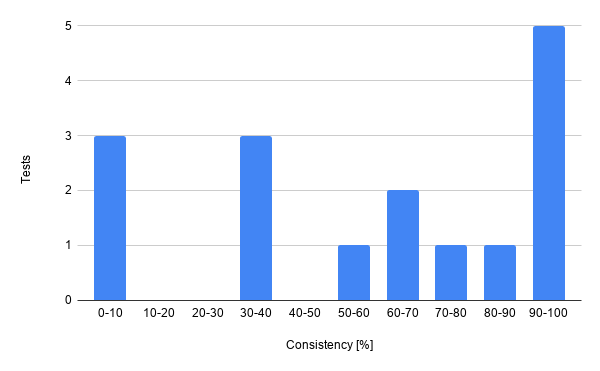
\includegraphics[width=\textwidth]{res/tests/data_hist_1.png}
        \caption{Consistency level histogram on key tests.}
        \label{fig:tests:data:hist_1}
    \end{figure}
    
    A high number of tests were successful, with 3 tests having an accuracy greater than 99\%.
    A value of 100\% is very difficult to achieve, since the data in the on-premise databases is downloaded at a different moment than that on the Data Warehouse.
    This difference can produce some false negative results, but they will always be related to a single day (usually the current one).
    As such, a value greater than 99\% can be considered an acceptable threshold.
    
    It was also shown that there were some inconsistencies between the two databases, but we were also able to identify their cause.
    Two tests failed because the required information had not been downloaded at all, one because hours had been remapped incorrectly, while the other failures were caused by a smaller date range.
    
    In the first case, the on-premise database contained information about specific countries or models, while the Data Warehouse contained information about different countries or models.
    This issue can usually be solved by a simple change in the downloader configuration.
    
    The two other problems were equally easy to solve.
    For the remappings, it was necessary to fix some values in the remapping table and rerun the procedure to materialize the correct values, while for the data range it was required to change the downloader configuration.
    
\paragraph{Value tests}
    Considering the acceptable results obtained with the Key tests, we decided to assess the correctness of the values.
    Out of 16 queries, 7 were related to forecasts, for which this kind of tests could not be applied.
    As a consequence, only the remaining 9 tests have been executed.
    
    \begin{figure}
        \centering
        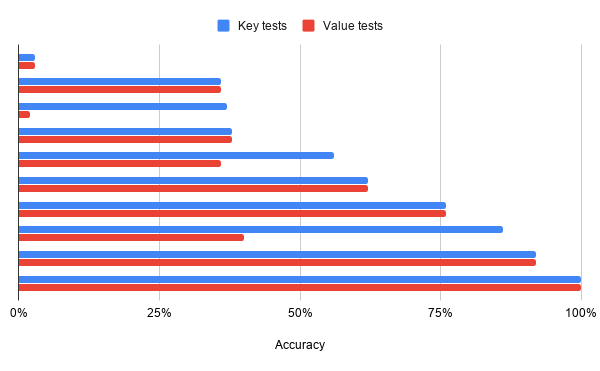
\includegraphics[width=\textwidth]{res/tests/data_val_1.png}
        \caption{Key-Value test results.}
        \label{fig:tests:data:value_1}
    \end{figure}
    
    The results, as shown in Figure \ref{fig:tests:data:value_1} were very positive, with 6 tests (66\% of the testing suite) having 100\% accuracy, while the others gave respectively 64\%, 47\% and 5\%.
    
    It should also be noted that in some cases the values stored in the on-premise databases were wrong, while those present in the Data Warehouse were correct.
    In these cases, it is impossible to perform an accurate analysis, and lower values are also accepted.
    This process is however carried out manually and these kind of exceptions are made for specific cases after a careful analysis.